\documentclass[./skripsi.tex]{subfiles}
\begin{document}
\chapter{Hasil Penelitian}
\section{Deskripsi Hasil Penelitian}
\par Hasil penelitian terdiri dari data hasil training CNN, LSTM, dan data hasil testing pada snortIDS
\par Data hasil pada sisi CNN melakukan filtrasi packet dengan mendeteksi packet yang berada dalam raw header. Sedangkan data hasil pada sisi LSTM melakukan profiling packet dengan memisahkan deret packet berdasarkan alamat IP yang kemudian dilakukan training.
\par Setiap input data langkah awal yang dilakukan adalah melakukan data mining untuk melihat sumber packet yang dikirim, dan tujuannya. Dan memprediksi apakah data itu masuk atau keluar.
\par Data yang dijadikan input pada sisi CNN adalah seluruh data yang masuk pada host. Sedangkan data yang dijadikan input pada sisi LSTM adalah seluruh data header baik keluar maupun masuk dari host.
\par Proses yang dilakukan untuk memperoleh data hasil adalah dengan menggunakan SnortIDS mengirimkan 10 parameter header dengan payloadnya. 
\par Pada sisi service flask akan didefinisikan buffer pada setiap data yang masuk berdasarkan sumber alamat IP nya. Buffer untuk IP ini terbagi menjadi 3 yakni, buffer transmit, receive, dan transceive. Buffer transmit, dan receive yang berkaitan akan digabungkan untuk mendeteksi intrusi pada sisi packet header dengan LSTM. Dan buffer transmit dengan per IP akan digunakan untuk mendeteksi intrusi pada sisi packet payload dengan CNN. 
\section{Hasil Training Data Neural Network}
\par Hasil training data untuk model Neural Network dengan model :
\subsection{Model CNN}
{\centering
\makebox {
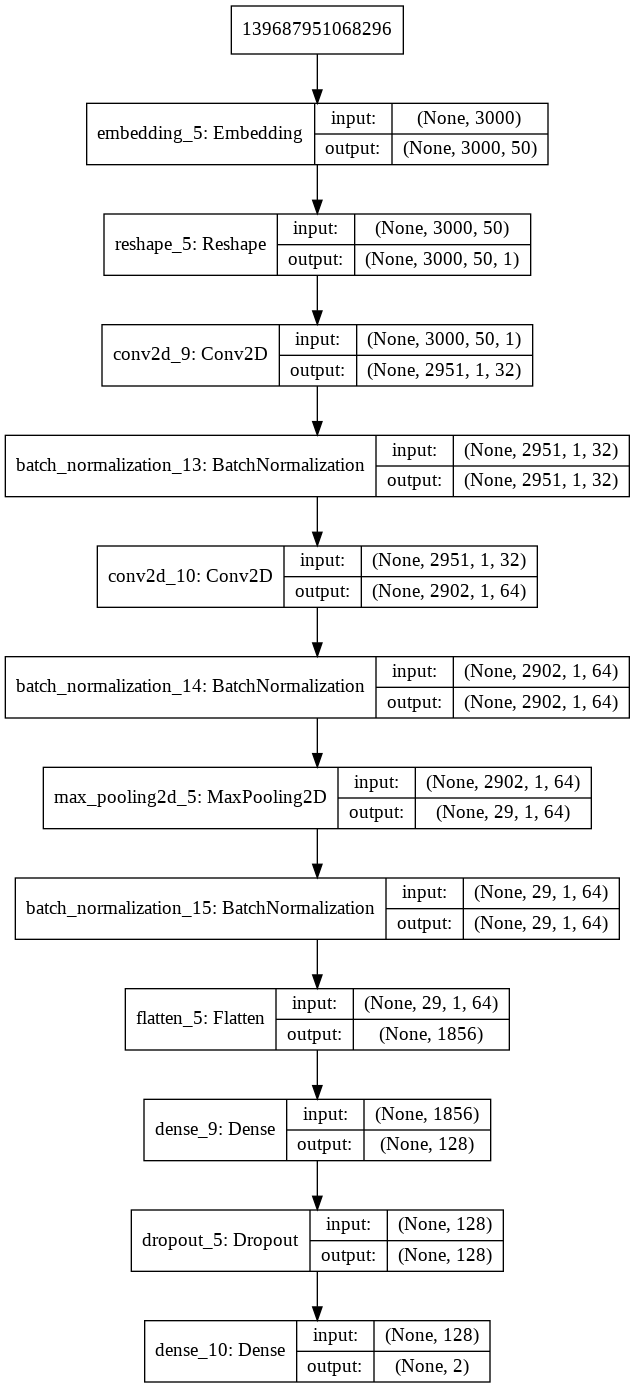
\includegraphics[width=0.5\textwidth]{skripsi/public/assets/img/CNNModel.png}
}
\captionof{figure}{Model CNN}\label{svc_loss}
}
\par Pada model CNN terdapat layer Embedding digunakan untuk mengekstraksi fitur dari data input dengan ukuran 2xMTU atau 3000 Byte. Layer selanjutnya adalah layer Reshape yang mengubah ukuran input dari 3000x50 menjadi 3000x50x1 dengan kata lain menginklusi matriks dari matriks 2 dimensi menjadi matriks 3 dimensi dengan ketebalan 1.
\par Layer selanjutnya merupakan layer konvolusi, pada konvolusi pertama dan kedua outputnya di normalisasi dengan BatchNormalization, dan pada Layers konvolusi terakhir dilakukan MaxPooling untuk meniadakan interpretasi yang akan mengurangi rate pendeteksian. Setelah semua konvolusi selesai matriks dinormalisasi lagi sebelum masuk ke layer selanjutnya.
\par Layer selanjutnya merupakan layer untuk deteksi. Pada layer Flatten semua matriks pada layer konvolusi terakhir diubah menjadi vektor. Kemudian setelah itu masuk ke layer Dense atau untuk aktivasi pertama lalu masuk ke Dropout untuk mengurangi neuron irrelevan dari Dense sebelumnya. Kemudian keluaran dari Dropout Layer menjadi input bagi Layer Dense terakhir yang berukuran vektor 2 bit, atau memiliki 2 kelas. Dari kedua kelas ini hanya kategori [0 1] yang dilakukan training data.

\subsection{Model LSTM}
{\centering
\makebox {
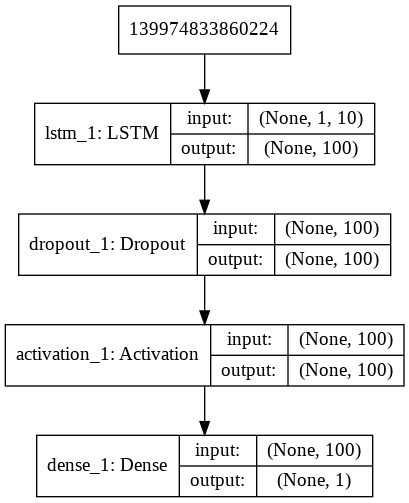
\includegraphics[width=0.5\textwidth]{skripsi/public/assets/img/LSTMModel.png}
}
\captionof{figure}{Model LSTM}\label{svc_loss}
}
\par Pada model LSTM hanya terdapat layer LSTM sebagai pembaca vektor header dari packet. Dropout untuk menghilangkan neuron yang irrelevan. Layer Activation dimana hasil keluaran Layer sebelumnya diaktivasi dengan menggunakan fungsi aktivasi \textit{softmax} dan Dense dengan ukuran klaster 1, yakni memiliki skalar untuk pendeteksiannya.
\par Untuk proses pendeteksian dengan sentiment analysis neuron Dense berjumlah 1, sedangkan untuk prediksi multivariable neuron Dense berjumlah 10, dimana neuron ini merupakan jumlah parameter pada header packet.
\subsection{Hasil Training Data LSTM}
\par Sistem training data LSTM menggunakan 2 metode yang berbeda yakni \textit{Sentiment Analysis} dan \textit{Multivariate Prediction}. Hasil \textit{training} kedua metode ini memiliki perbedaan dimana pada \textit{Sentiment Analysis} dapat memprediksi apabila variasi dan distribusi variasi pada targetnya merata. Sedangkan pada \textit{Multivariate Prediction} hasil training memiliki karakteristik konvergen yang tinggi karena memperhitungkan dan memprediksi data secara keseluruhan.
\subsubsection{Hasil training SVCHOSTA Botnet dengan Sentiment Analysis LSTM}
\makebox{
\centering
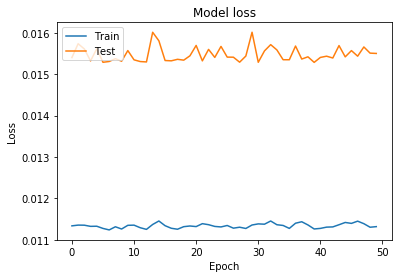
\includegraphics[width=\textwidth]{skripsi/public/assets/img/svc_loss.png}
}
\captionof{figure}{Loss svchosta model LSTM}\label{svc_loss}
Dari data diatas dapat dilihat konvergensi loss pada sisi training tidak mempengaruhi loss pada sisi testing. Hal ini disebabkan karena data yang bernilai malicious pada \textit{header} sangat kecil sehingga dapat diabaikan.
\makebox{
\centering
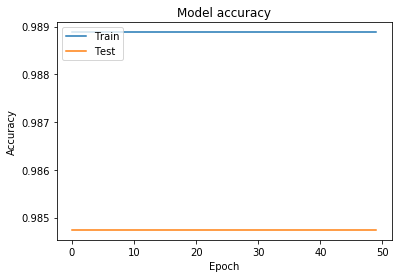
\includegraphics[width=\textwidth]{skripsi/public/assets/img/svc_acc.png}
}
\captionof{figure}{Akurasi svchosta model LSTM }\label{svc_acc}
Dari data diatas dapat dilihat sesuai dengan nilai sebelumnya. Hal ini disebabkan karena data yang bernilai malicious pada \textit{header} sangat kecil sehingga dapat diabaikan.
\subsubsection{Hasil Training Neris Botnet dengan Sentiment Analysis LSTM}
\makebox{
\centering
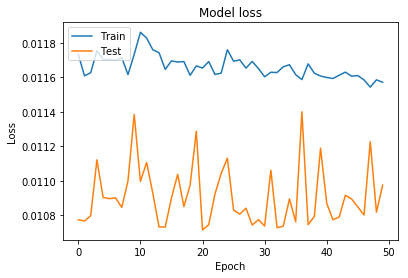
\includegraphics[width=\textwidth]{skripsi/public/assets/img/neris_loss.png}
}
\captionof{figure}{Loss Neris model LSTM}\label{neris_loss}

\makebox{
\centering
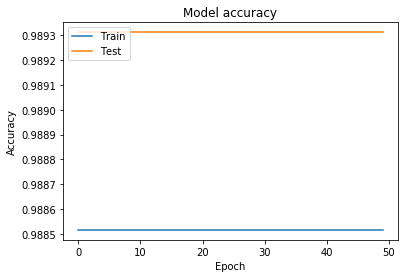
\includegraphics[width=\textwidth]{skripsi/public/assets/img/neris_acc.png}
}
\captionof{figure}{Akurasi Neris model LSTM}\label{neris_acc}

\subsubsection{Hasil Training Rbot Botnet dengan Sentiment Analysis LSTM}
\makebox{
\centering
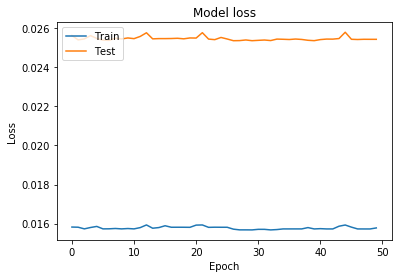
\includegraphics[width=\textwidth]{skripsi/public/assets/img/rbot_loss.png}
}
\captionof{figure}{Loss Rbot model LSTM}\label{rbot_loss}

\makebox{
\centering
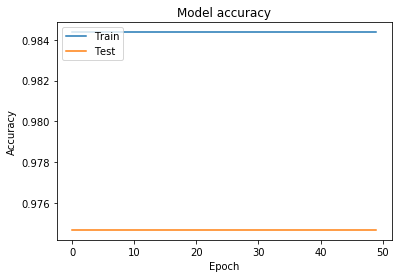
\includegraphics[width=\textwidth]{skripsi/public/assets/img/rbot_acc.png}
}
\captionof{figure}{Akurasi Rbot model LSTM}\label{rbot_acc}

\subsubsection{Hasil traiing SVCHOSTA Botnet dengan Multivariate Prediction LSTM}
\makebox{
\centering
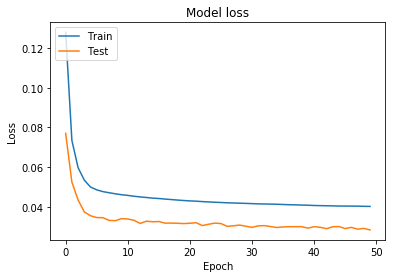
\includegraphics[width=\textwidth]{skripsi/public/assets/img/svc2_loss.png}
}
\captionof{figure}{Loss svchosta model LSTM}\label{svc2_loss}

\makebox{
\centering
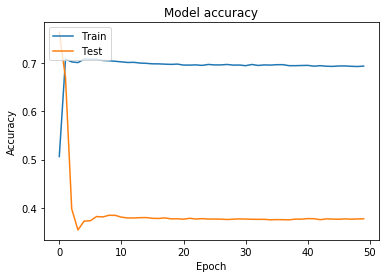
\includegraphics[width=\textwidth]{skripsi/public/assets/img/svc2_acc.png}
}
\captionof{figure}{Akurasi svchosta model LSTM }\label{svc2_acc}

\subsubsection{Hasil Training Neris Botnet dengan Multivariate Prediction LSTM}
\makebox{
\centering
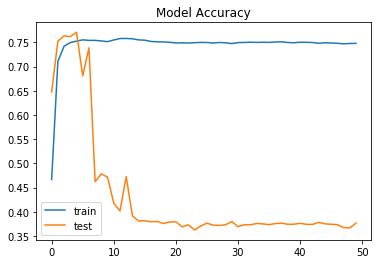
\includegraphics[width=\textwidth]{skripsi/public/assets/img/neris2_loss.png}
}
\captionof{figure}{Loss Neris model LSTM}\label{neris2_loss}

\makebox{
\centering
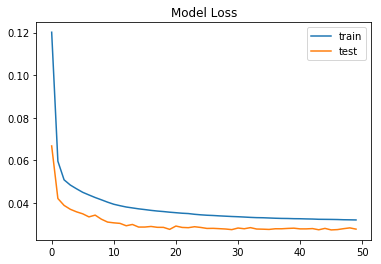
\includegraphics[width=\textwidth]{skripsi/public/assets/img/neris2_acc.png}
}
\captionof{figure}{Akurasi Neris model LSTM}\label{neris2_acc}

\subsubsection{Hasil Training Rbot Botnet dengan Multivariate Prediction LSTM}
\makebox{
\centering
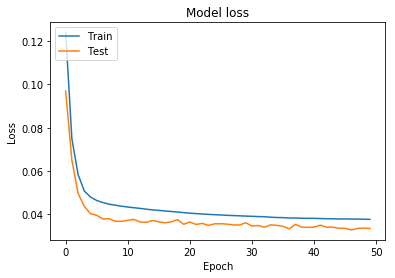
\includegraphics[width=\textwidth]{skripsi/public/assets/img/rbot2_loss.png}
}
\captionof{figure}{Loss Rbot model LSTM}\label{rbot2_loss}

\makebox{
\centering
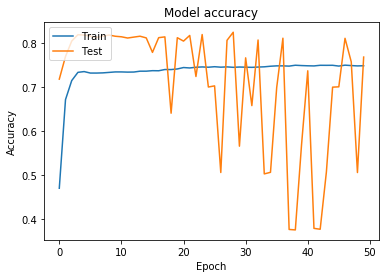
\includegraphics[width=\textwidth]{skripsi/public/assets/img/rbot2_acc.png}
}
\captionof{figure}{Akurasi Rbot model LSTM}\label{rbot2_acc}

\subsection{Hasil Training Data CNN}
\par Pada sistem ini, training data CNN menggunakan matriks konvolusi 1D. Hal ini dilakukan untuk melihat keterikatan satu dengan yang lain dengan faktor jarak relatif pada sampel input.
\subsubsection{Hasil Training CNN Pada BotNet Neris}
\makebox{
\centering
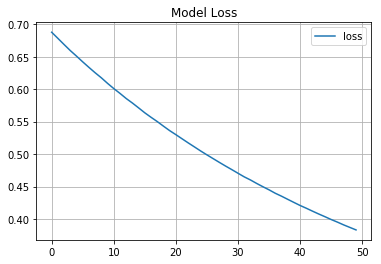
\includegraphics[width=\textwidth]{skripsi/public/assets/img/cnn_neris_loss.png}
}
\captionof{figure}{Model Loss CNN Neris}\label{cnn_neris_loss}

\makebox{
\centering
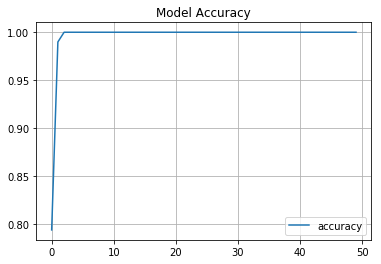
\includegraphics[width=\textwidth]{skripsi/public/assets/img/cnn_neris_acc.png}
}
\captionof{figure}{Model Accuracy CNN Neris}\label{cnn_neris_acc}

\subsubsection{Hasil Training CNN Pada BotNet RBot}
\makebox{
\centering
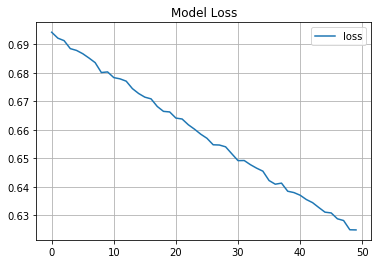
\includegraphics[width=\textwidth]{skripsi/public/assets/img/cnn_rbot_loss.png}
}
\captionof{figure}{Model Loss CNN RBot}\label{cnn_rbot_loss}

\makebox{
\centering
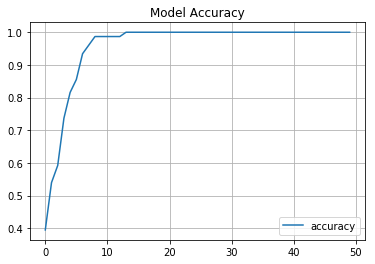
\includegraphics[width=\textwidth]{skripsi/public/assets/img/cnn_rbot_acc.png}
}
\captionof{figure}{Model Accuracy CNN RBot}\label{cnn_rbot_acc}

\subsbusection{Hasil Training CNN Pada BotNet Svchosta}
\makebox{
\centering
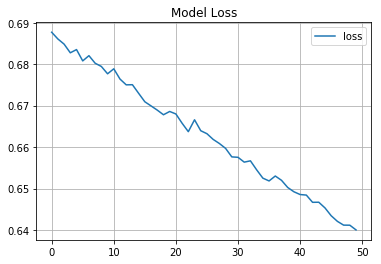
\includegraphics[width=\textwidth]{skripsi/public/assets/img/cnn_svchosta_loss.png}
}
\captionof{figure}{Model Loss CNN SVCHosta}\label{cnn_svchosta_loss}

\makebox{
\centering
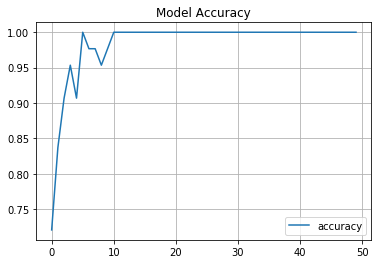
\includegraphics[width=\textwidth]{skripsi/public/assets/img/cnn_svchosta_acc.png}
}
\captionof{figure}{Model Accuracy CNN SVCHosta}\label{cnn_svchosta_acc}

\subsubsection{Hasil Training CNN Pada Single Type}
\makebox{
\centering
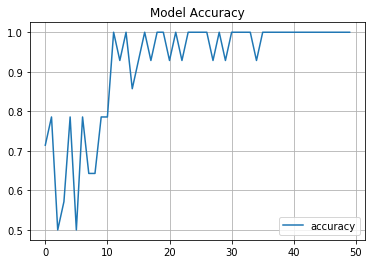
\includegraphics[width=\textwidth]{skripsi/public/assets/img/cnn_single_acc.png}
}
\captionof{figure}{Model Accuracy CNN Single type}\label{cnn_single_acc}

\subsbusection{Hasil Training CNN Pada BotNet Svchosta}
\makebox{
\centering
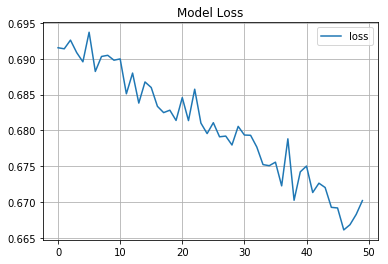
\includegraphics[width=\textwidth]{skripsi/public/assets/img/cnn_single_loss.png}
}
\captionof{figure}{Model Loss CNN Single Type}\label{cnn_single_loss}

\subsubsection{Hasil Training CNN Pada Multi Virus}
\makebox{
\centering
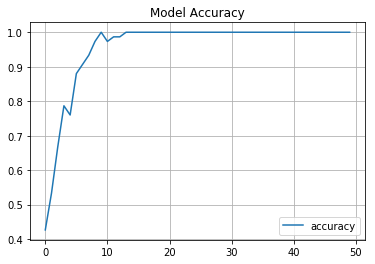
\includegraphics[width=\textwidth]{skripsi/public/assets/img/cnn_multi_acc.png}
}
\captionof{figure}{Model Accuracy CNN Single type}\label{cnn_multi_acc}

\subsbusection{Hasil Training CNN Pada BotNet Svchosta}
\makebox{
\centering
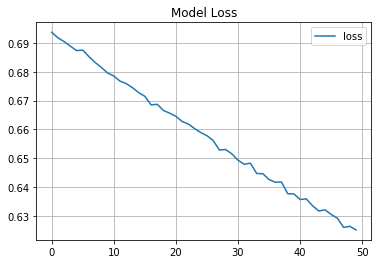
\includegraphics[width=\textwidth]{skripsi/public/assets/img/cnn_multi_loss.png}
}
\captionof{figure}{Model Loss CNN Multi Type}\label{cnn_multi_loss}

\section{Hasil Testing Data Neural Network}
\subsection{Hasil Testing Data LSTM}
\par Testing dilakukan dengan mengeksport bobot dari LSTM dan menggunakannya pada preprocessor yang telah dibuat pada SnortIDS.
Sistem LSTM ini melakukan testing pada data header pada tiap \textit{network packet} yang masuk pada NIC.
\par Rancangan LSTM untuk analisis \textit{network packet header} ini dapat di implementasikan pada snort lebih dari 1 bobot LSTM saja. Pada setiap bobot bisa diberikan label untuk memberitahukan data bobot LSTM ini digunakan untuk memprediksikan apa.
\subsection{Hasil Testing Data CNN}
\par Testing dilakukan dengan mengeksport bobot dari CNN dan menggunakannya pada preprocessor yang telah dibuat pada SnortIDS. CNN berperan sebagai \textit{filter} untuk memfiltrasi \textit{network packet} yang masuk apakah mengandung malware atau tidak.
\par CNN Filter ini digunakan untuk memfiltrasi \textit{Payload} dari \textit{network packet} untuk mencegah terjadinya penyebaran virus dan malicious software lainnya.
\par CNN Filter ini memiliki 2 target untuk menentukan sistem filtrasi yang dipakai apakah \textit{Whitelist} target 0, atau \textit{Blacklist} target 1.
\par Filter CNN ini juga dapat digunakan dengan banyak bobot, dan setiap bobotnya dapat diberikan label untuk memberitahukan untuk apa bobot ini digunakan.
\par Sistem Filtrasi dijalankan secara asinkron dengan cara melakukan passing Payload kepada \textit{Service} Filter yang dijalankan, kemudian \textit{Service} tersebut mengirim dalam bentuk \textit{response} nilai target, untuk menentukan apakah \texit{payload} ini aman.
\end{document}